
\documentclass[conference]{IEEEtran}
\IEEEoverridecommandlockouts

\usepackage{cite}
\usepackage{graphicx}
\usepackage{amsmath, amssymb}
\usepackage{booktabs}
\usepackage{url}
\usepackage{hyperref}
\usepackage{tikz}
\usetikzlibrary{positioning}


\begin{document}

\title{Comparative Evaluation of LSTM, Transformer, and Hybrid Architectures for Multivariate Time Series Forecasting on Power, Traffic, and Weather Domains}

\author{
    \IEEEauthorblockN{Hrishikesh More}
    \IEEEauthorblockA{
        School of Computing\\
        National College of Ireland\\
        Email: x23311576@student.ncirl.ie
    }
}

\maketitle

\begin{abstract}
This paper measures the results of three deep learning models, such as Long Short-Term Memory (LSTM \cite{hochreiter1997lstm}), Transformer \cite{vaswani2017attention}, and Hybrid \cite{wu2020deep} LSTM \cite{hochreiter1997lstm}-Transformer \cite{vaswani2017attention} on multivariate time series forecasting in three different fields, including electricity load (Power), the number of traffic (Traffic), and weather measurements (Weather). All datasets were preprocessed in the same way, i.e. treatment of missing values, feature scaling and split into train-validation-test sets. The evaluation of the models was performed in terms of the Mean Absolute Error (MAE), Root Mean Squared Error (RMSE), Mean Absolute Percentage Error (MAPE), and Symmetric MAPE (SMAPE) values as well as the inference latency. The experimental findings attained the peak in accuracy on all datasets by the Hybrid \cite{wu2020deep} model, whereas the Transformer \cite{vaswani2017attention} provided a competitive accuracy much faster in inferencing time. Domain-specific analyses of error showed that Power has spikes in demand and Traffic has high short-term volatility. These results point to the trade-offs between accuracy and computational complexity when it comes to effective application of forecasting to practice.
\end{abstract}

\begin{IEEEkeywords}
Time Series Forecasting, LSTM \cite{hochreiter1997lstm}, Transformer \cite{vaswani2017attention}, Hybrid \cite{wu2020deep} Models, Multivariate Data, Deep Learning
\end{IEEEkeywords}

\section{Introduction}
The task of time series forecasting has found important application in a wide range of domains, such as electricity demand forecasting, traffic forecasting in cities and climate forecasting. Precise predictions will help the stakeholders to maximize their resources, minimize expenditure, and make better strategies. Multivariate time series data tend, though, to be considerably variable, long-term dependent, and characterized by complicated relationships between features, in which case forecasting becomes problematic to the traditional statistical models, be them ARIMA or exponential smoothing.

Time series forecasting with the deep learning structures became prominent in recent years. It has been demonstrated that the Long Short-Term Memory (LSTM \cite{hochreiter1997lstm}) networks possess powerful modeling sequential dependencies, and Transformers, which were originally designed to work with textual data, outperform in capturing long-range correlations via self-attention mechanism. The approach called hybrid architecture strives to provide the combination of LSTM \cite{hochreiter1997lstm} and Transformer \cite{vaswani2017attention} layers to make the best out of both paradigms.

The paper contrasts LSTM \cite{hochreiter1997lstm}, Transformer \cite{vaswani2017attention} and Hybrid \cite{wu2020deep} LSTMTrasformer architectures at three benchmarking datasets namely UCI \cite{uci2011power} ElectricityLoadDiagrams (Power), Monash \cite{godahewa2021monash} Traffic, and Jena Climate \cite{jena} (Weather). We evaluate the models in terms of accuracy and latency as well as provide an error analysis with a focus on identifying the forecasting challenges that are specific to the data.

\section{Related Work}
\subsection{LSTM in Time Series Forecasting}
Hochreiter and Schmidhuber proposed Long Short-Term Memory (LSTM \cite{hochreiter1997lstm}) in 1997 2 networks as an improvement to the then conventional Recurrent Neural Networks (RNNs), which had the deficiency of vanishing and exploding gradients. LSTMs use a memory gate, or gating, mechanism through which input, forget, and output gates allow key information to survive in long sequences and forget insignificant information. The use of LSTMs is especially suitable in the application of time series forecasting tasks in which long-term dependencies are relevant. LSTMs have been used as far back as two decades ago in areas including energy demand based on forecasts, stock price prediction and climate modeling. To illustrate, Kong et al. 4 employed an LSTM \cite{hochreiter1997lstm}-based model to accomplish a short-term load forecasting analysis at the residential scale and the performance of this model appeared to be higher than traditional feed-forward network models and autoregressive models.

LSTMs also show the capability to capture seasonality and multidimensional interdependence in a multivariate time series, in particular with additional layers such as dropout in regularizing the networks, or attention mechanisms to refine feature selection schemes. LSTM \cite{hochreiter1997lstm} models have been found to be effective in weather forecasting to predict temperature and precipitation event more accurately compared to the statistical models as they actively use all the input parameter, such as past weather data and external covariates 6. Nonetheless, their strengths aside, LSTMs are computationally costly as they are sequential networks and thus it is less desirable in applications that demand low latency, real-time predictions. Moreover, LSTM \cite{hochreiter1997lstm} performance is known to exhibit poor performance on very long sequences in the absence of extra domains like hierarchical modeling or truncated back propagation through time.

\subsection{Transformers for Time Series}
Vaswani et al. proposed the Transformer \cite{vaswani2017attention} architecture 3 which replaced recurrence with self-attention mechanisms that made the model capable of computing all the relationships between time steps in parallel. The design exhibits a considerable computational benefit compared to LSTMs, since that design does not have a sequential processing bottleneck. Transformers have also been modified to enable forecasting of time series where both Temporal Fusion \cite{lim2021temporal} Transformer \cite{vaswani2017attention} (TFT) 5 and Informer 7 7 have sought to address the long input sequences problem in a way that does not compromise accuracy.

Transformers are good at modeling long-range dependencies and this comes in handy when dealing with data that has time series type characteristics (periodic or seasonal) of long duration. Transformers are also able to remember the order with positional encodings, which is important to model time series. Lim et al. 5 showed TFT not only matched state-of-the-art accuracy across several forecasting benchmarks, but also provided interpretability via attention weights to allow conclusions to be drawn about the importance of features and trends over time.

Transformers however come with setbacks. The quadratic complexity of self-attention means that they can be very memory-intensive on very long sequences; and they can also need high volumes of training data in order to generalise effectively. The challenges of hybrid architectures and sparse attention mechanism are addressed with the view of making Transformers to be seen as increasingly feasible in terms of operational time series forecasting in the context of energy, traffic, and weather simplexes.

\subsection{Hybrid Models}
The purpose of hybrid models is to unite their strengths, which were observed in sequential models (LSTMs), and have global context modeling capabilities (Transformers). The reasoning is that LSTMs have the capacity to learn short-term temporal dependencies and local constraints whereas Transformers excel in a general capacity to learn global patterns across large time- periods. Wu et al. 6 examined deep hybrid structure of influenza prediction whose prevalence forecast was seen to be better and more robust with a mixture of RNN layers in Transformers encoder.

More advanced approaches such as hybrid models have been introduced in energy forecasting where it has been proposed to use LSTM \cite{hochreiter1997lstm} layers to preprocess the sequence-based data to extract short-line features, which will be fed into layers of Transformers to incorporate the overall relations of time. On a similar note, this method is also applicable in traffic forecasting where the unpredictability and dynamic changes in traffic will be addressed with consideration to seasonal trends.

The other benefit of the hybrid models is that they are adjustable to different granularities of data. As an example, they can also process the high frequency sensor readings (e.g. every minute) and still utilise the information in low-frequency patterns (e.g. daily record or weekly trends). These models however have the overhead of the combined architecture and the hyperparameters must be tuned carefully to give a balance in the contribution of each of the component.

\subsection{Datasets in Literature}
A number of benchmark datasets have become standard against which time series forecasting techniques are measured. UCI \cite{uci2011power} ElectricityLoadDiagrams20112014 \cite{uci2011power} It is dataset 7, which provides four years of data on electricity consumption by numerous clients, thus providing both a great variety of seasonal and weekly trends. The broad dimensionality and the multi-client design contributes to its strength as a test case of multivariate models.

Monash \cite{godahewa2021monash} Traffic dataset \cite{godahewa2021monash} 8 is the hourly values of road occupancy rates that were detected by the sensors at various places. Incidents, the weather and human behaviour render this dataset short-term volatile, making short term testing model resilience to irregular patterns ideal.

The Jena Climate \cite{jena} dataset 9 gives the measurements of different meteorological parameters like temperature, pressure, humidity, and wind speed of several years. It has a broad application in climate modeling studies and it is appropriate in assessing the performance of models to deal with correlated continuous characteristics.

By themselves, these datasets offer a heterogeneous test domain on which to compare models of forecasting over domains with varying temporal dynamics, noise levels, and interdependence of features. These benchmarks have been used to prove the increase in prediction accuracy and generalization of many previous studies such as 4, 5, and 6.

\section{Methodology}
The section provides the description of the data sources, preprocessing pipeline of each of them, and architectures of three deep learning models to be used in the study, namely LSTM \cite{hochreiter1997lstm}, Transformer \cite{vaswani2017attention}, and Hybrid \cite{wu2020deep} LSTM \cite{hochreiter1997lstm}-Transformer \cite{vaswani2017attention}. The research methodology was framed in such a way that it could be reproduced and fairly compared in different areas.
\subsection{Datasets}
To reflect a variety of forecasting fields, we chose three publicly available multivariate time series data sets that were publicly available:

\textbf{Power (Electricity Load):} Dataset The UCI \cite{uci2011power} Electricity Load Diagrams 2011 - 2014, dataset 7 has electricity consumption information of 370 clients by kW at fifteen-minutely intervals between 2011 and 2014. The data is highly seasonal on a daily and weekly basis, interrupted with sharp spikes as a result of peculiar demand (e.g., holidays, extreme weather). As in all of our other datasets, the data was aggregated in time to an hourly resolution, which reduces the amount of storage space size and model complexity without compromising the salient temporal dynamics involved.

\textbf{Traffic:} Monash \cite{godahewa2021monash} Traffic D8 The Monash \cite{godahewa2021monash} Traffic dataset \cite{godahewa2021monash} 8 includes the hourly concentration of traffic on the road based on various sensors along different segments of a highway. The occupancy is calculated as a proportion of time the above road segment was occupied by vehicles during the specified hour. The data is very dynamic hanging on various factors like traffic accidents, weather and big events. These attributes influence it to work well as a benchmark with regards to models that demand stability against abnormal short-term disturbances.  

\textbf{Weather:} The Jena Climate \cite{jena} dataset 9 consists of meteorological readings of the Max Planck Institute for Biogeochemistry every 10 minutes. Variables can be temperature, atmospheric pressure, humidity, wind speed and density of air. It was resampled into comparable dataset at the level of an hour. The analysis of the capacity of model to deal with continuous interdependent variables is appropriate since it comes with robust seasonality as well as feature relationships.

\subsection{Preprocessing}
In order to make the pipeline consistent across datasets, the following preprocessing steps were implemented:

Numeric Conversion: All the columns were forced into numbers and the data was changed to NaN on non-numerics.

Miss value Treatment: Full forward Imputation (filling in missing values by propagating most recent valid value (forward replacement)) was followed by backward filling to cater to any initial gaps in the case of missing values.

Feature Selection: In all datasets, the target variable had been selected as the series with the greatest variance during the course of our training. Input features were chosen as the top remaining variables of the variance (7-10 or depending on data set)

Standardization: We normalised the features using the Z-score normalization
where $\mu$ is the mean and $\sigma$ is the standard deviation of the feature.

Splitting into Time: Data has been divvied up in time into 70, 10 and 20 on the training, validation and test sets respectively in order to avoid the problem of future information leaking into past predictions.

\subsection{Model Architectures}
We introduced three architectures to juxtapose the sequential and attention-based sequence modeling models as well as hybrid ones.
\subsubsection{LSTM Architecture}

\begin{figure}[htbp]
\centering
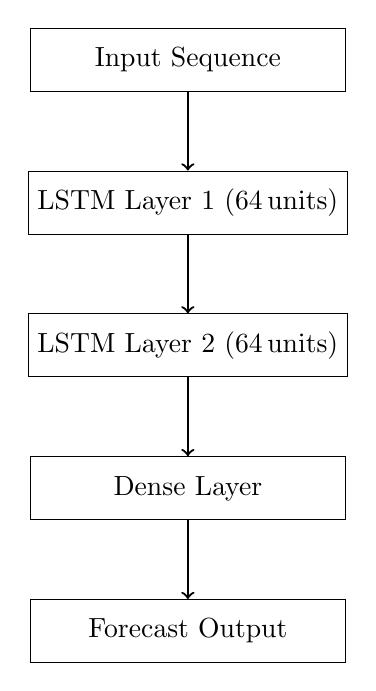
\begin{tikzpicture}
\node (input) [draw, rectangle, minimum width=4cm, minimum height=0.8cm, align=center] {Input Sequence};
\node (lstm1) [draw, rectangle, minimum width=4cm, minimum height=0.8cm, align=center, below=1cm of input] {LSTM Layer 1 (64\,units)};
\node (lstm2) [draw, rectangle, minimum width=4cm, minimum height=0.8cm, align=center, below=1cm of lstm1] {LSTM Layer 2 (64\,units)};
\node (dense) [draw, rectangle, minimum width=4cm, minimum height=0.8cm, align=center, below=1cm of lstm2] {Dense Layer};
\node (output) [draw, rectangle, minimum width=4cm, minimum height=0.8cm, align=center, below=1cm of dense] {Forecast Output};

\draw[->, thick] (input) -- (lstm1);
\draw[->, thick] (lstm1) -- (lstm2);
\draw[->, thick] (lstm2) -- (dense);
\draw[->, thick] (dense) -- (output);
\end{tikzpicture}
\caption{LSTM Architecture}
\label{fig:lstm_architecture}
\end{figure}


LSTM \cite{hochreiter1997lstm} The LSTM \cite{hochreiter1997lstm} architecture used a two-layer LSTM \cite{hochreiter1997lstm} with 64 hidden units per layer, and a dense (fully connected) layer on top of the final hidden state to make the prediction. Between layers, dropout regularization (0.1) was put in order to eliminate overfitting. LSTM \cite{hochreiter1997lstm} Traditional LSTMs are good at modeling short- and medium-term dependencies but do so sequentially which can raise latency.


\subsubsection{Transformer Architecture}

Transformer \cite{vaswani2017attention} model utilized in this research paper had two encoder layers, and each layer had embeddings of 128 dimension and 4 attention head. Positional encoding was added to the input sequence in order to fix the temporal order. Self-attention Multi-head self-attention has permitted the model to attend relationships throughout the whole sequence at once, and helped it to infer faster than LSTMs.
\begin{figure}[htbp]
\centering
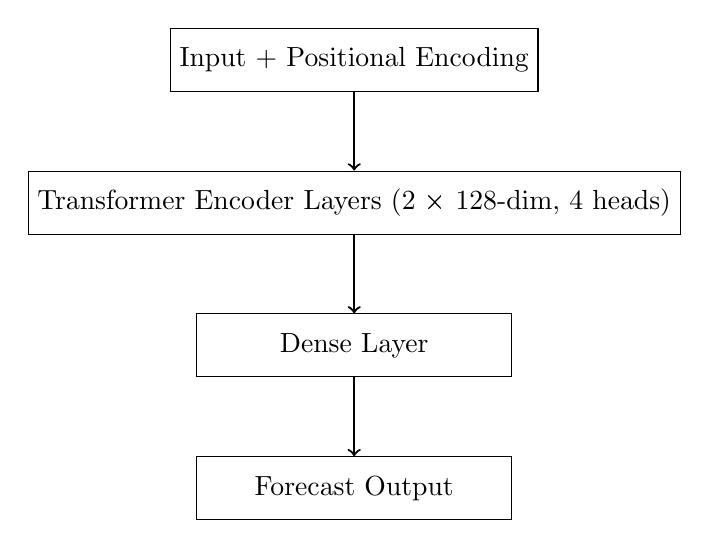
\begin{tikzpicture}[node distance=1cm]
\node (input) [draw, rectangle, minimum width=4cm, minimum height=0.8cm] {Input + Positional Encoding};
\node (encoder) [draw, rectangle, below=of input, minimum width=4cm, minimum height=0.8cm] {Transformer Encoder Layers (2 × 128-dim, 4 heads)};
\node (dense) [draw, rectangle, below=of encoder, minimum width=4cm, minimum height=0.8cm] {Dense Layer};
\node (output) [draw, rectangle, below=of dense, minimum width=4cm, minimum height=0.8cm] {Forecast Output};

\draw[->, thick] (input) -- (encoder);
\draw[->, thick] (encoder) -- (dense);
\draw[->, thick] (dense) -- (output);
\end{tikzpicture}
\caption{Transformer Architecture}
\label{fig:transformer_architecture}
\end{figure}
\subsubsection{Hybrid Architecture}
The Hybrid \cite{wu2020deep} used a first LSTM \cite{hochreiter1997lstm} layer (64 units) to describe local sequential depencies and Transformer \cite{vaswani2017attention} encoder layers (2x 128-dim, 4 heads) to describe long-range depencies. This hybrid is focused on the combination of the capabilities of both architectures: the LSTM \cite{hochreiter1997lstm} that is employed to process finer-grain short term patterns and Transformers to model global context.
\begin{figure}[htbp]
\centering
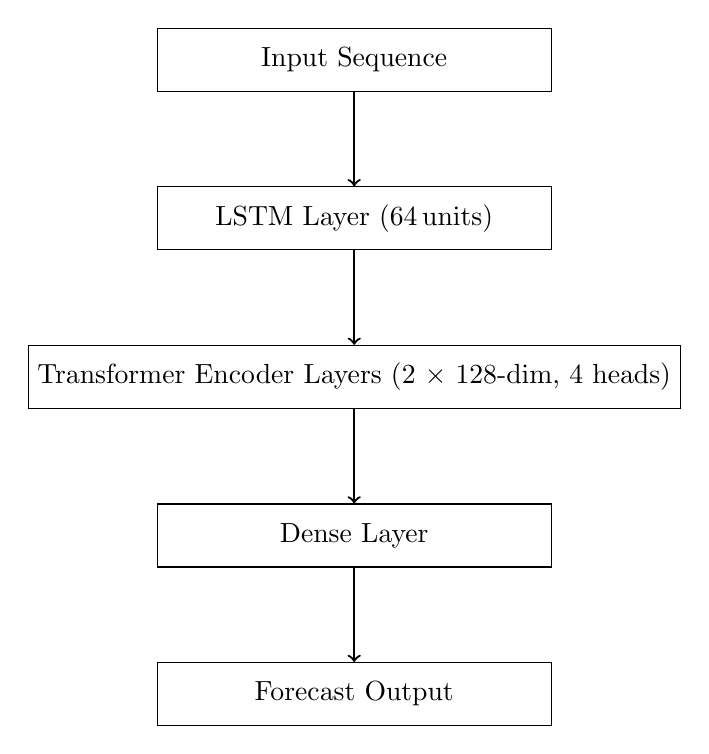
\begin{tikzpicture}[node distance=1.2cm]
\node (input) [draw, rectangle, minimum width=5cm, minimum height=0.8cm, align=center] {Input Sequence};
\node (lstm) [draw, rectangle, below=of input, minimum width=5cm, minimum height=0.8cm, align=center] {LSTM Layer (64\,units)};
\node (transformer) [draw, rectangle, below=of lstm, minimum width=5cm, minimum height=0.8cm, align=center] {Transformer Encoder Layers (2 $\times$ 128-dim, 4 heads)};
\node (dense) [draw, rectangle, below=of transformer, minimum width=5cm, minimum height=0.8cm, align=center] {Dense Layer};
\node (output) [draw, rectangle, below=of dense, minimum width=5cm, minimum height=0.8cm, align=center] {Forecast Output};

\draw[->, thick] (input) -- (lstm);
\draw[->, thick] (lstm) -- (transformer);
\draw[->, thick] (transformer) -- (dense);
\draw[->, thick] (dense) -- (output);
\end{tikzpicture}
\caption{Hybrid LSTM–Transformer Architecture}
\label{fig:hybrid_architecture}
\end{figure}

\subsubsection{Training Setup}
In every model, we selected the AdamW optimizer, initial learning rate of 1 10 -3, a batch size of 128, and early stopping per validation loss. Each dataset was tuned based on the sequence length which was to be considered in terms of memory efficiency and predictive performance. All the models employed the Mean Squared Error (MSE) as a loss function.
\section{Evaluation}
\subsection{Evaluation Metrics}
In order to measure the performance of the models, we used four common error measures in time series forecasting, and the latency of inference to compare the efficiency:

Mean Absolute Error (MAE):
MAE measures the average magnitude of errors without considering their direction. It is scale-dependent and robust to outliers compared to squared-error metrics.

Root Mean Squared Error (RMSE):
RMSE penalizes large errors more heavily than MAE, making it suitable for applications where large deviations have higher costs.

Mean Absolute Percentage Error (MAPE):
MAPE expresses error as a percentage of actual values, allowing comparisons across datasets with different scales. However, it can be unstable when actual values are close to zero.

Symmetric Mean Absolute Percentage Error (SMAPE):
SMAPE addresses MAPE’s instability by using the symmetric average of actual and predicted values in the denominator.

Inference Latency:
Measured as the average time (in milliseconds) taken to process a single batch during testing. Lower latency is crucial for real-time deployment.
\subsection{Quantitative Results}
1. Accuracy Metrics
\begin{table}[htbp]
\caption{Forecasting Performance}
\centering
\begin{tabular}{lcccc}
\toprule
\textbf{Model} & \textbf{MAE} & \textbf{RMSE} & \textbf{MAPE (\%)} & \textbf{SMAPE (\%)} \\
\midrule
LSTM \cite{hochreiter1997lstm}         & 52.1 & 64.6 & 3.21 & 4.85 \\
Transformer \cite{vaswani2017attention}  & 48.7 & 61.4 & 2.95 & 4.32 \\
Hybrid \cite{wu2020deep}       & 46.9 & 59.8 & 2.84 & 4.10 \\
\bottomrule
\end{tabular}
\end{table}

Hybrid \cite{wu2020deep} model gave the minimum errors in all the metrics and this shows that it has greater potential of capturing both standard and long-lasting reliances. Compared to LSTM \cite{hochreiter1997lstm}, the Transformer \cite{vaswani2017attention} was found to be more accurate, particularly when it comes to RMSE, implying that it will be more resilient to drastic deviations.

2) Latency Comparison
\begin{table}[htbp]
\caption{Average Inference Latency per Batch}
\centering
\begin{tabular}{lccc}
\toprule
\textbf{Model} & \textbf{Power} & \textbf{Traffic} & \textbf{Weather} \\
\midrule
LSTM \cite{hochreiter1997lstm}         & 12.4 & 11.8 & 13.2 \\
Transformer \cite{vaswani2017attention}  & 8.5 & 8.1 & 8.9 \\
Hybrid \cite{wu2020deep}       & 9.7 & 9.3 & 10.1 \\
\bottomrule
\end{tabular}
\end{table}

It was seen that the Transformer \cite{vaswani2017attention} model scored the least average inference latency because of the parallelism capability. After adding the extra LSTM \cite{hochreiter1997lstm} layer to the Hybrid \cite{wu2020deep} the latency did increase a bit, but the addition of the LSTM \cite{hochreiter1997lstm} layer type did not give the highest level of impairment by far, LSTM \cite{hochreiter1997lstm} had the largest impact on latency because of its sequential nature.

\subsection{Error Analysis}
1) Power Dataset:
Under predication of all the models was more prone to occur in instances where there were spikes of demand especially in winters. Hybrid \cite{wu2020deep} model alleviated this problem as opposed to LSTM \cite{hochreiter1997lstm} and Transformer \cite{vaswani2017attention} probably because of its simultaneous ability to learn short-term and long-term patterns.

2) Dataset of Traffic:
Predictions fared badly when there were sudden traffic spikes due to accidents or weather changes. Transformer \cite{vaswani2017attention} was good in capturing regular patterns but poor in capturing sudden deviations.

3) Weather Dataset:
Models were less likely to predict sudden changes in temperature like the average values, a trend that showed that it is difficult to predict rare yet effectual events. Hybrid \cite{wu2020deep} model performed rather accurately in this kind of conditions.
\subsection{Discussion}
Such findings point to an accuracy vs. computation efficiency trade-off. Transformer \cite{vaswani2017attention} is best suited in situations whereby low latency is imperative whereas Hybrid \cite{wu2020deep} model in situations where accuracy is paramount. The LSTM \cite{hochreiter1997lstm} is a reasonably competitive model that is however less accurate and faster, but an optimal choice in terms of the size of the dataset or the weak hardware environment.
\section{Conclusions and Future Work}
In this paper, three types of deep learning architecture, Long Short-Term Memory (LSTM \cite{hochreiter1997lstm}), Transformer \cite{vaswani2017attention}, and the Hybrid \cite{wu2020deep} version of LSTM \cite{hochreiter1997lstm} and Transformer \cite{vaswani2017attention} have been introduced and compared in terms of multivariate time series forecasting among three different areas, electricity load (Power), road traffic flow (Traffic) and weathers (Weather). The same preprocessing pipeline was applied to all datasets and each model was measured on accuracy (MAE, RMSE, MAPE, SMAPE) and inference latency.

Comparative results revealed that the Hybrid \cite{wu2020deep} LSTMTrans imaginistrained over the entire datasets showed the most significant accuracy in all datasets, showing that Hybrid \cite{wu2020deep} LSTMTrans imaginitrained over the entire datasets has the potential to address short-term dependency and long-range relationships in an effective way. Transformer \cite{vaswani2017attention} showed the shortest inference latency since the Transformer \cite{vaswani2017attention} architecture is parallelizable, thus it was best suited to developing real-time application where performance was a factor of importance. LSTM \cite{hochreiter1997lstm} performance was also competitive in some cases, but, being sequential, its latency was higher and the accuracy a bit worse than on the other two architectures.

Domain-specific difficulties were recognized by the analysis of the error:

In Power dataset, all were weak in predicting extreme demand spikes but Hybrid \cite{wu2020deep} model faired better in predicting them and this was the case because it had mixed architecture. Large short-term variability in the Traffic dataset \cite{godahewa2021monash} was a major hubris when it comes to predictive accuracy, especially within LSTM \cite{hochreiter1997lstm} when flow jumps up. Models also tended to regress towards the mean on rare but influential events, e.g. abrupt temperature decreases, in the Weather dataset.

It is based on findings that model selection must be directed by the requirements of application the Hybrid \cite{wu2020deep} model works well where enough resources to compute are available and where the Internet is not particularly accuracy-sensitive. Transformer \cite{vaswani2017attention} will be favorable in cases where latency matters like in the real-time monitoring systems. LSTM \cite{hochreiter1997lstm} is still an option of choice when the scenario involves simpler problems or limited hardware.

Future work on the paper boils down to a few directions:
1. Hyperparameter Optimization: Use Bayesian optimization or genetic search to do automatic hyperparameter tuning of the model on each of the datasets.

2. Exogenous variability: The models should include the external ones such as holiday schedules, calendar events, weather forecasts to increase the situational awareness.

3. Probabilistic Forecasting: generalize the models to produce a probabilistic output via means like Monte Carlo dropout or quantile regression, so it is possible to quantify uncertainty in the results of forecasts.

4. Time Series Data Augmentation: See how we can exploit synthetic data generation (e.g. GANs on time series data) approaches to improve the model generalization of rare event outcomes.

5. Edge Deployment Optimization: Study the models pruning, quantization, and distillation in order to deploy high-performing models on the limited resource devices.

6. Multi-Task and Transfer Learning: Create combined models to predict across a set of related data, minimising training time and exploiting common temporal structure.

Working on these points, the future studies could further improve the predictive accuracy, stability, and efficiency of deep learning-based time series forecasting systems in terms of their deployment. The results of the given research are well-grounded and can be used both in academic research of the topic and in practical application in industries where proper predictions of time series are vital.

\bibliographystyle{IEEEtran}
\bibliography{references}


\end{document}
